\documentclass{beamer}
\usepackage{graphicx}
\usepackage{hyperref}
\usetheme{Boadilla}
\title{Commodity Price Analysis Through PCA, KNN, and Neural Nets}
\subtitle{for Corn and Soybeans}
\author{Joe Nunez}
\institute{Harvey Mudd College}
\date{May 25, 2018}

\begin{document}
\begin{frame}
\titlepage
\end{frame}

\begin{frame}
\frametitle{Data Set}
\begin{itemize}
\item The data set I used was taken from Kaggle.com and from Quandl.com, and consisted of monthly economic data concerning corn and soybeans from 2007 to 2014, as well as futures market data for corn and soybean prices over the same period.
\item The economic data included 112 different indicators related to corn and 69 different indicators related to soybean data, including figures on imports, exports, total area planted/harvested, regional production figures, and the size of regional reserves. 

\item The market data consisted of daily measures of market open, high, low, close, volume, and open interest for the futures contracts.
\end{itemize}
\end{frame}


\begin{frame}
\frametitle{Data Set}
\begin{itemize}
\item The economic data was gathered from the USDA's monthly World Agricultural Supply and Demand Estimate (WASDE).
\item The market data was gathered from Quandl.com
\end{itemize}
\end{frame}


\begin{frame}
\frametitle{Methods --- Labeling}
\begin{itemize}
\item I took two approaches: one using the market data alone and one using the economic data.
\item For both data sets, I used the prices from the market data to determine whether the price of the given commodity (corn or soybeans) went up or down in a given time step.  If the price did go up, that data point was labeled true, and if it did not, it was labeled false.  
\item I also labeled the data with its price at the next timestep for use in regression.
\item For market data, the time step was one day, and for WASDE data, the time step was one week.
\end{itemize}
\end{frame}

\begin{frame}
\frametitle{Methods --- Features}
\begin{itemize}
\item For the economic data, the feature vector was simply all of the entries provided in the WASDE report, after being normalized to all be between 0 and 1 (subtracting by the minimum, then dividing by the difference between min and max).
\item For the market data, the feature vector consisted of open, high, low, close, volume, and open interest for each of the previous 22 days.
\end{itemize}
\end{frame}

\begin{frame}
\frametitle{Methods --- PCA-KNN}
\begin{itemize}
\item Principal component analysis was used for all number of features from 1 to 40.
\item $k$ nearest neighbors was used to classify the points resulting from PCA, with values of $k$ ranging from 2 to 30.
\item Plots will not show higher numbers of components or values of $k$ because they did not show higher performance.
\item Sklearn packages were used for both PCA and KNN.
\end{itemize}
\end{frame}

\begin{frame}
\frametitle{Methods --- Neural Network}
\begin{itemize}
\item Layers of size [256, 256, 32, 1]
\item Using sigmoid activation function.
\item Used LSTM for market data, where the LSTM layers were the first two layers.
\item Used a multi-layer perceptron for WASDE data.
\item Neural networks were implemented using Keras.
\end{itemize}
\end{frame}

\begin{frame}
\frametitle{Previously --- PCA, Corn, WASDE}
\begin{center}
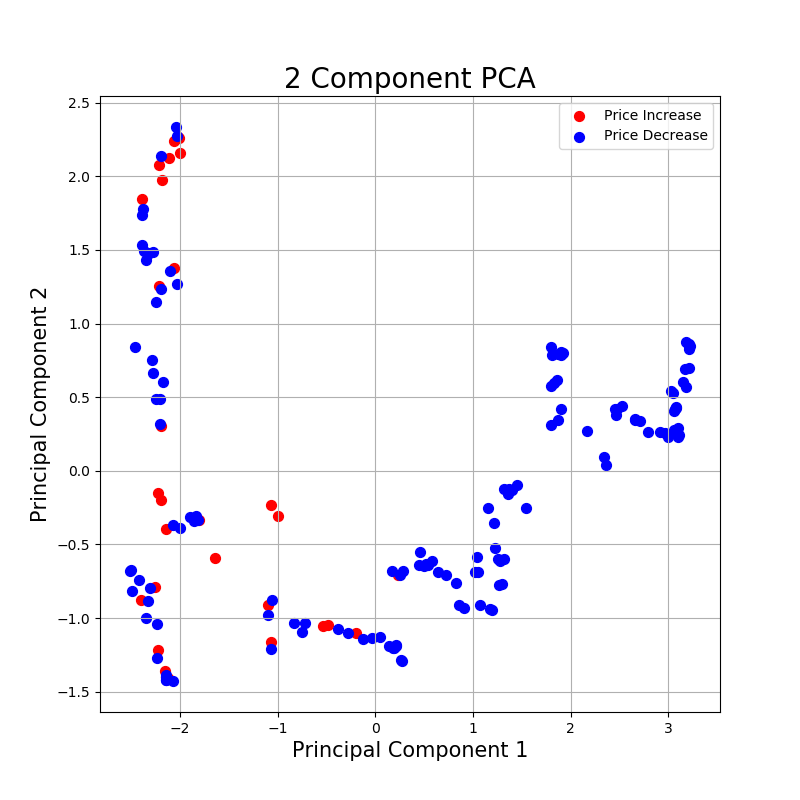
\includegraphics[scale=.4]{images/fullcorn}
\end{center}
\end{frame}

\begin{frame}
\frametitle{Previously --- PCA, Corn, Market}
\begin{center}
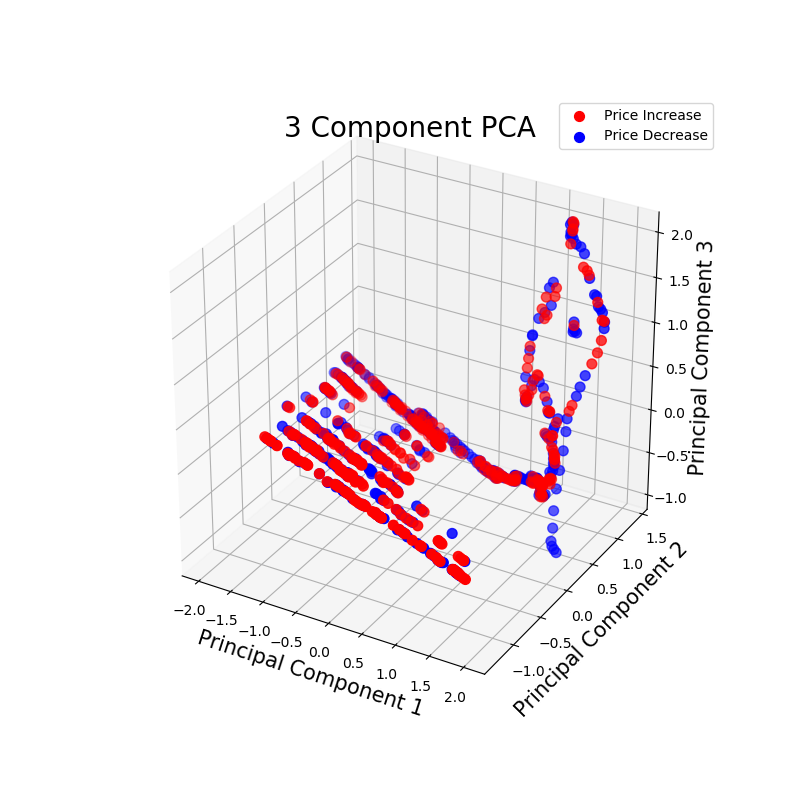
\includegraphics[scale=.4]{images/cornmkt5,3d}
\end{center}
\end{frame}

\begin{frame}
\frametitle{Results --- PCA-KNN, Corn, WASDE}
\begin{center}
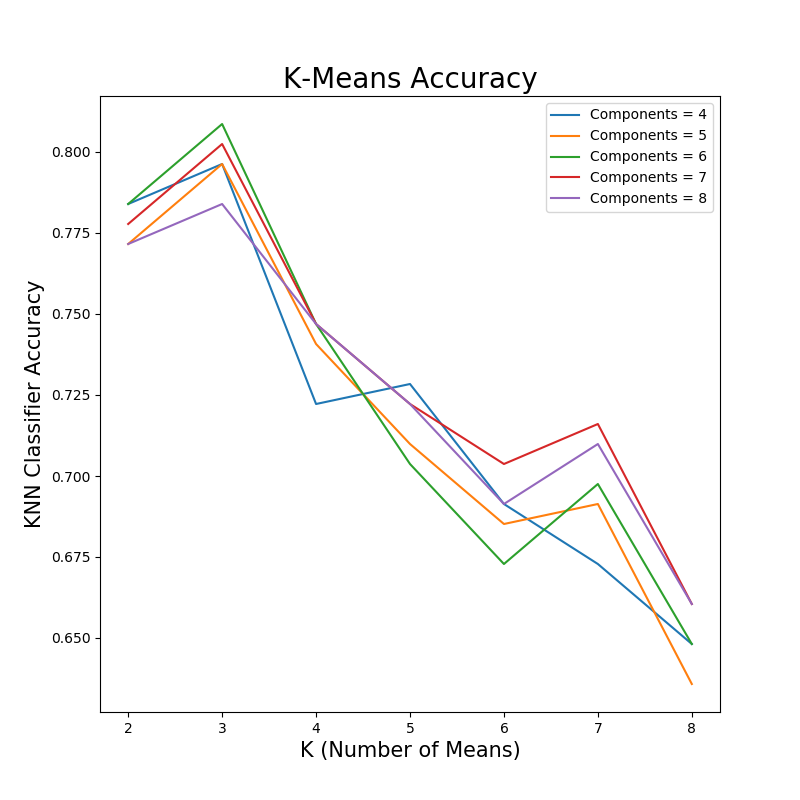
\includegraphics[scale=.4]{images/cornacc4,8,w}
\end{center}
\end{frame}

\begin{frame}
\frametitle{Results ---  PCA-KNN, Soybeans, WASDE}
\begin{center}
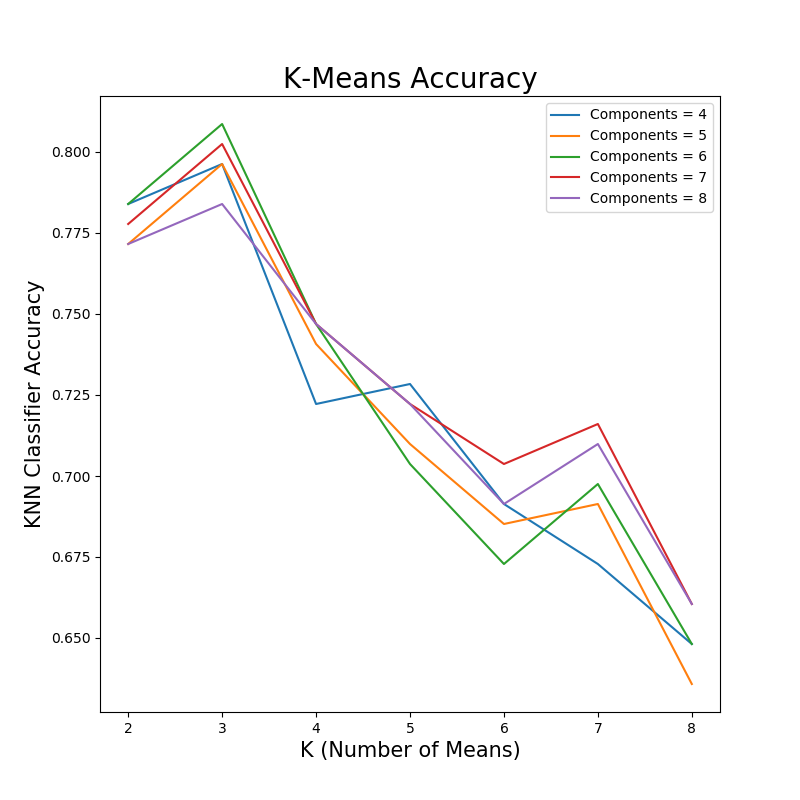
\includegraphics[scale=.4]{images/soyacc4,8,w}
\end{center}
\end{frame}

\begin{frame}
\frametitle{Results ---  PCA-KNN, Corn, Market}
\begin{center}
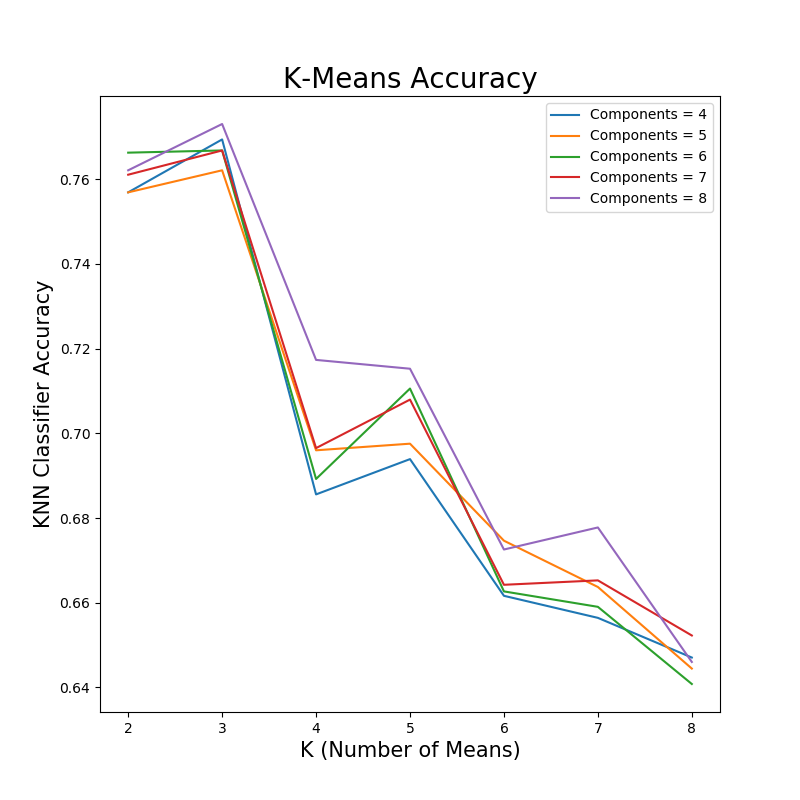
\includegraphics[scale=.4]{images/cornacc4,8,m}
\end{center}
\end{frame}

\begin{frame}
\frametitle{Results ---  PCA-KNN, Soybeans, Market}
\begin{center}
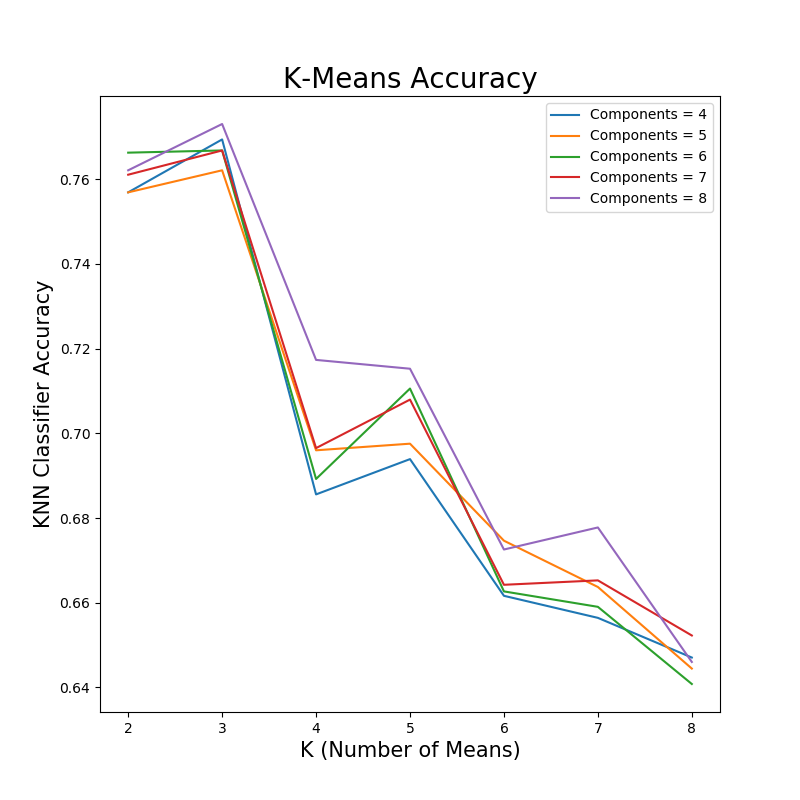
\includegraphics[scale=.4]{images/soyacc4,8,m}
\end{center}
\end{frame}

\begin{frame}
\frametitle{Results --- MLP Prediction, Corn, WASDE}
\begin{center}
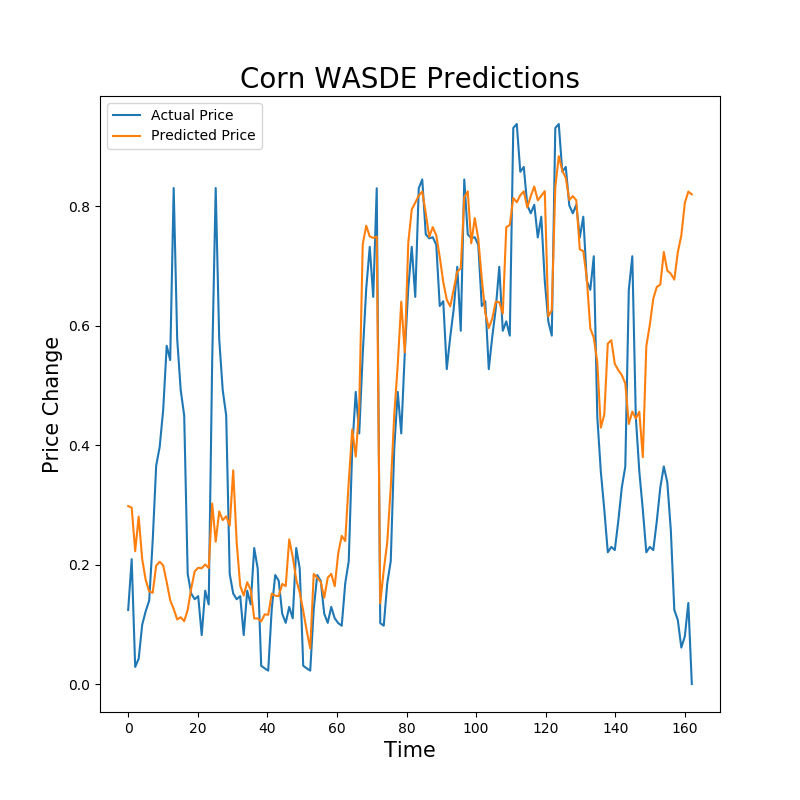
\includegraphics[scale=.4]{images/CornWASDE}
\end{center}
\end{frame}

\begin{frame}
\frametitle{Results --- MLP Prediction, Soybeans, WASDE}
\begin{center}
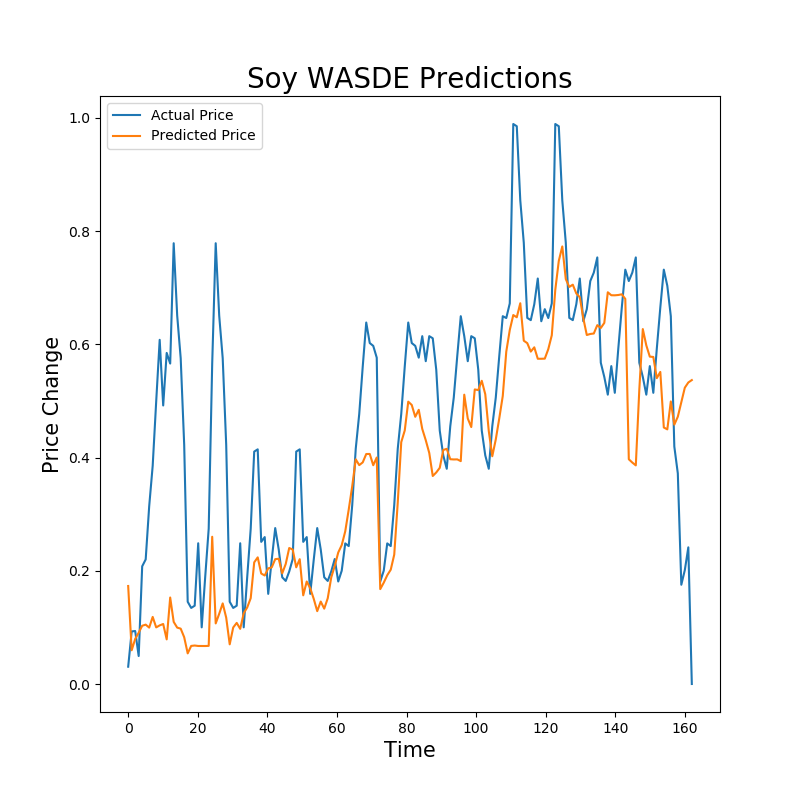
\includegraphics[scale=.4]{images/SoyWASDE}
\end{center}
\end{frame}

\begin{frame}
\frametitle{Results --- LSTM Prediction, Corn, Market}
\begin{center}
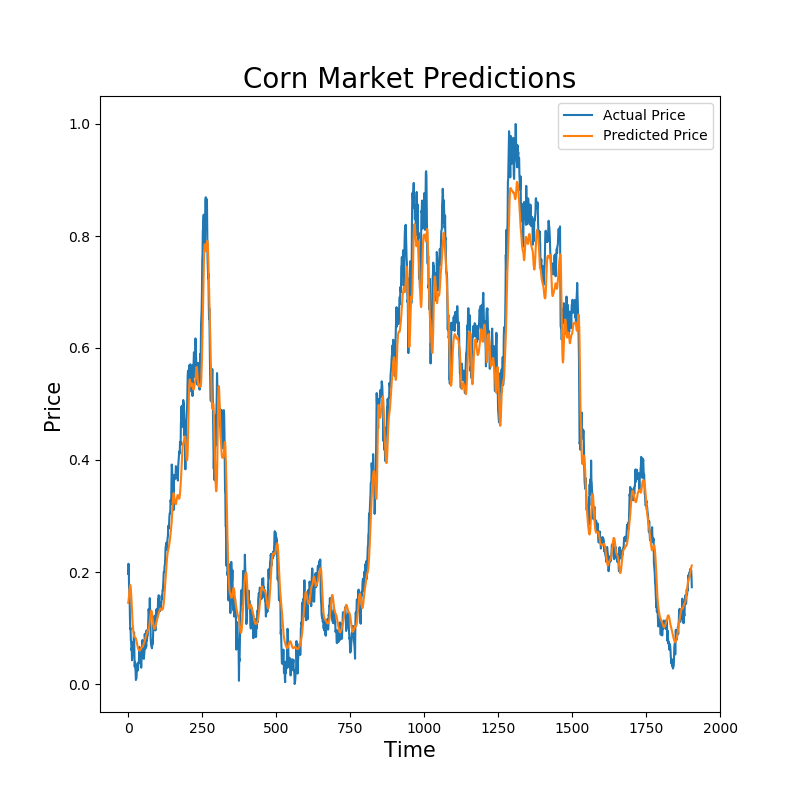
\includegraphics[scale=.4]{images/CornMarket}
\end{center}
\end{frame}


\begin{frame}
\frametitle{Results --- LSTM Prediction, Soybeans, Market}
\begin{center}
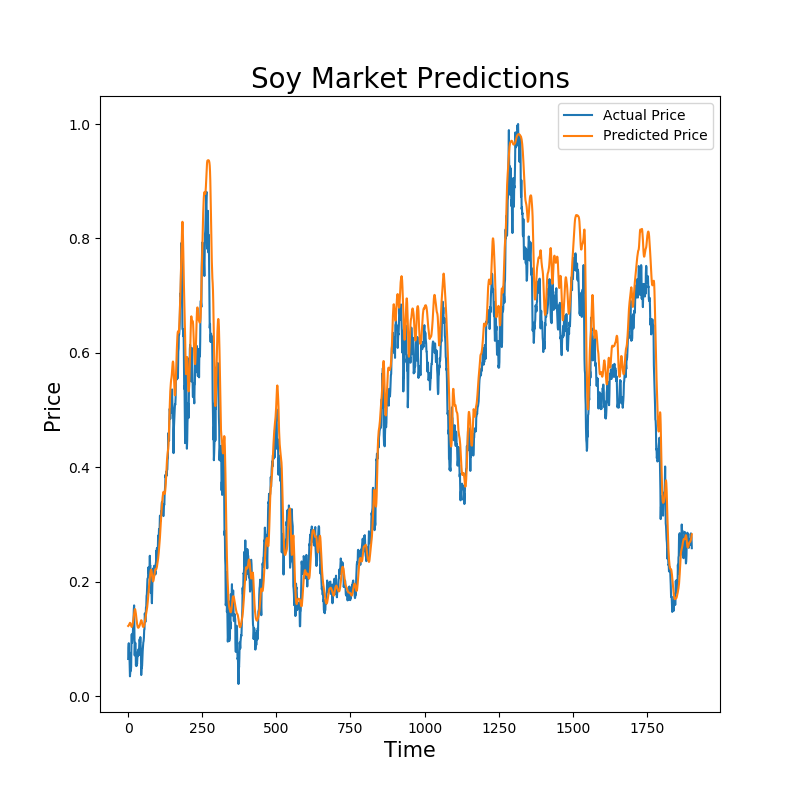
\includegraphics[scale=.4]{images/SoyMarket}
\end{center}
\end{frame}



\begin{frame}
\frametitle{Results}
\begin{itemize}
\item As we can see for the prediction plots, the neural nets are not especially good at guessing the price, but do generally get the trend of the price (up or down) correct. 
\item If we scan through the predictions, we can see what percentage of the time the predicted price direction matches the actual price direction.
\end{itemize}
\end{frame}

\begin{frame}
\frametitle{Results}
\begin{itemize}
\item WASDE Corn MLP Accuracy: 61.3\%
\item WASDE Soybean MLP Accuracy: 54.8\%
\item Market Corn LSTM Accuracy: 49.9\%
\item Market Soybean LSTM Accuracy: 51.2\%

\end{itemize}
\end{frame}




\begin{frame}
\frametitle{Conclusions}
\begin{itemize}

\item The ability to detect these trends may not be as significant as they appear.  The trends may be the result of seasonal trends, which commodities futures contracts often price in, so this knowledge may not be actionable.
\item Incorporating futures prices versus spot prices for a contract may serve as a better labeling system, though it would require data I did not have time to gather.
\item It is possible that the WASDE data may provide better results under a convolutional model, which will better factor in which elements of the WASDE report are most important for a prediction.

\end{itemize}

\end{frame}



\begin{frame}
\frametitle{Conclusions}
\begin{itemize}

\item It is possible that day-long time intervals between market data samples are too long for an LSTM to be able to extract meaningful trends.  Markets may simply be too volatile over the course of single day for daily data to provide significant information.  It is possible that incorporating intraday pricing will improve performance.

\item It is likely that a more sophisticated neural should be able to provide accuracy in the 80\% range.  In particular, softmax activation functions coupled with convolutional layers may provide comparable performance to PCA-KNN, since convolutional layers have been proved to be equivalent to PCA and softmax may provide a similar categorization effect to KNN.

\end{itemize}
\end{frame}


\begin{frame}
\frametitle{Questions?}
Sources:
\vspace{.1in}
\\Data 
\\\url{https://www.kaggle.com/ainslie/usda-wasde-monthly-corn-soybean-projections}
\\\url{https://www.q uandl.com}
\vspace{.1in}
\\Coding
\\\url{https://github.com/mGalarnyk/Python_Tutorials/blob/master/Sklearn/PCA/PCA_Data_Visualization_Iris_Dataset_Blog.ipynb}
\end{frame}













\end{document}